\section{Modello di sviluppo iniziale} \label{section:modello_di_sviluppo}
Inizialmente il gruppo ha deciso di lavorare secondo il \textbf{modello incrementale} per il \textit{ciclo di vita}\glo{} del software per i seguenti motivi:
\begin{itemize}
  \item Può produrre valore ad ogni incremento, aiutando a fissare meglio i requisiti per gli incrementi successivi;
  \item Ogni incremento riduce il rischio di fallimento;
  \item Le funzionalità principali sono sviluppate nei primi incrementi, rendendole via via più stabili.
\end{itemize}
Nel modello incrementale i requisiti vengono classificati in base alla loro importanza strategica. In questo modo, quelli più importanti vengono
trattati prima. Questo ne aumenta la chiarezza e la facilità di soddisfazione. I requisiti meno importanti invece vengono soddisfatti in seguito,
venendo così inseriti in un sistema già stabilizzato.\\
Il metodo di lavoro sarà quindi il seguente:
\begin{itemize}
  \item In ogni fase di lavoro vengono prefissati degli incrementi che devono essere prodotti entro una scadenza decisa dal gruppo;
  \item Il lavoro viene diviso tra i membri del gruppo;
  \item Al termine del periodo prefissato, servirà una riunione per analizzare il lavoro svolto da ogni membro, riscontrare problemi e difficoltà;
  \item Sarà compito dei \textit{verificatori} controllare il lavoro svolto dagli altri membri del gruppo e sollevare eventuali incongruenze o errori;
  \item Alla fine di questa verifica, seguirà una nuova discussione di gruppo per stabilire se gli obiettivi dell'incremento sono stati soddisfatti.
\end{itemize}

\begin{figure}[H]
  \centering
  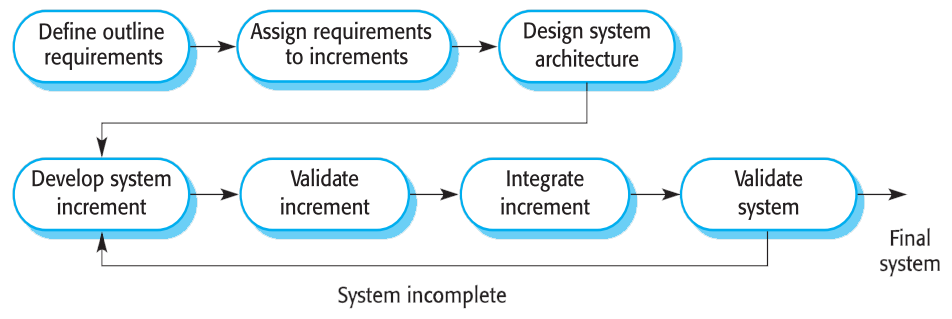
\includegraphics[scale=0.6]{immagini/modello_incrementale.png}
  \caption{Modello incrementale - tratto da: Ian Sommerville, \textit{Software Engineering}, 8th ed.}
\end{figure}
\pagebreak

%%%%%%%%%%%%%%%%%%%%%%%%%%%%%%%%%%%%%%%%%%%%%%%%%%%%%%%%%%%%%%%%%%%%%%%%%%%

\subsection{Incrementi individuati} \label{subsection:incrementi}
In seguito è riportata la tabella con indicati gli incrementi individuati, con il rispettivo obiettivo e i requisiti e casi d'uso ad esso associati.
I requisiti riportati includono tutti i requisiti figli. Tutti i requisiti non riportati sono da intendersi soddisfatti, in parte, da
ogni incremento. \\
Ogni requisito e caso d'uso è definito tramite il suo codice identificativo, per maggiori informazioni fare riferimento all'\docNameVersionAdR{}.

\begin{table}[H]
  \centering
  \renewcommand{\arraystretch}{1.8}
  \rowcolors{2}{green!100!black!40}{green!100!black!30}
  \begin{tabular}{c|p{6cm}|c|c}
    \rowcolor[HTML]{125E28}
    \color[HTML]{FFFFFF}\textbf{Incr.}
        & \multicolumn{1}{c}{\color[HTML]{FFFFFF}\textbf{Obiettivo}}
        & \multicolumn{1}{c}{\color[HTML]{FFFFFF}\textbf{Requisiti}}
        & \multicolumn{1}{c}{\color[HTML]{FFFFFF}\textbf{Casi d'uso}}                                                                                                                                                                 \\
    \hline
    I   & Studio di Fantom\glo{} come blockchain\glo{} di riferimento e relative differenze con Ethereum\glo{}, studio del linguaggio Solidity\glo{} e relativi ambienti di sviluppo. & \Shortunderstack{R1V1, R1V2,                  \\R2V4, R1V6,\\R1V10, R1V11\\} & - \\
    II  & Studio di tecnologie, librerie e pattern per lo sviluppo Frontend\glo{} di React.                                                                                           & \Shortunderstack{R1V3, R3V5,                  \\R1V7, R1V8,\\R1V9, R1V12,\\R1V13\\} & - \\
    %%%%%%%
    III & Stesura smart contract\glo{} per pagamento singolo e relativo modulo frontend\glo{} per l'interazione tramite Metamask\glo{}.                                               & \Shortunderstack{R1F1, R1F2,                  \\R1F2.1, R1F3,\\R1F4, R1F5,\\R1F5.1, R1F5.3,\\R1F5.4, R1F7,\\R1F8\\} & \Shortunderstack{UC1, UC2.1,\\UC2.2, UC2.2.1,\\UC2.3, UC2.3.1,\\UC2.3.3, UC2.4,\\UC4, UC6,\\UC7\\}\\
    IV  & Studio e realizzazione del design con esaltazione dei diversi cambiamenti di stato.                                                                                         & \Shortunderstack{R1F11, R1F11.1,              \\R1F11.2, R1F13,\\R1F14, R1F14.1,\\R1F14.2, R1F14.3,\\R1F14.4\\} & \Shortunderstack{UC2.3.4, UC4,\\UC4.1, UC4.2,\\UC4.3, UC5,\\UC5.1, UC5.3\\}\\
    V   & Aggiunta di funzionalità Rimborso nello smart contract\glo{} e relativo modulo frontend\glo{} per l'interazione tramite Metamask\glo{}.                                     & R1F6                               & UC8, UC9 \\
    %%%%%%%
    VI  & Aggiunta di funzionalità MoneyBox\glo{} nello smart contract\glo{} e relativo modulo frontend\glo{} per l'interazione tramite Metamask\glo{}.                               & \Shortunderstack{R2F2.2, R2F2.2.1,            \\R2F2.2.2, R2F2.2.4,\\R2F2.2.5, R2F5.2,\\R1F15\\} & \Shortunderstack{UC2.2.2, UC2.2.3,\\UC2.3.2, UC3.1,\\UC3.2, UC3.3,\\UC8, UC9\\}\\
  \end{tabular}
\end{table}
\begin{center}
  \textit{\small Continua nella pagina successiva}
\end{center}
\begin{table}[H]
  \centering
  \renewcommand{\arraystretch}{1.8}
  \rowcolors{2}{green!100!black!40}{green!100!black!30}
  \begin{tabular}{c|p{6cm}|c|c}
    \rowcolor[HTML]{125E28}
    \color[HTML]{FFFFFF}\textbf{Incr.}
         & \multicolumn{1}{c}{\color[HTML]{FFFFFF}\textbf{Obiettivo}}
         & \multicolumn{1}{c}{\color[HTML]{FFFFFF}\textbf{Requisiti}}
         & \multicolumn{1}{c}{\color[HTML]{FFFFFF}\textbf{Casi d'uso}}                                                                                                               \\
    \hline
    VII  & Aggiunta di Ricerca, Paginazione e Filtrazione dell'elenco delle transazioni per maggiore fruibilità.                            & \Shortunderstack{R2F8.1, R2F8.1.1,     \\R2F8.1.2, R2F8.1.3,\\R1F8.2, R2F8.2.1,\\R2F8.2.2, R2F8.2.3,\\R2F8.2.4\\} & \Shortunderstack{UC7.1, UC7.1.1,\\UC7.1.2, UC7.1.3,\\UC7.2, UC7.2.1,\\UC7.2.2, UC7.2.3,\\UC7.2.4\\} \\
    VIII & Aggiunta funzione dello smart contract\glo{} per la conversione del denaro in stable coin\glo{}.                                 & R2F9                               & - \\
    IX   & Integrazione funzionalità d'identificazione grafica per i dati presenti in blockchain\glo{} e sviluppo punti opzionali restanti. & \Shortunderstack{R3F2.2.3, R3F10,      \\R3F12\\} & UC3.5 \\
  \end{tabular}
  \caption{Incrementi individuati}
\end{table}
\pagebreak

%%%%%%%%%%%%%%%%%%%%%%%%%%%%%%%%%%%%%%%%%%%%%%%%%%%%%%%%%%%%%%%%%%%%%%%%%%%

\section{Modello di sviluppo attuale} \label{section:modello_di_sviluppo_attuale}
A seguito delle considerazioni fatte dal prof. Vardanega durante la revisione \RTB{} il gruppo, dopo una riunione interna, ha deciso di attuare delle importanti modifiche a quello che è il nostro modello di sviluppo.\\
Dopo una attenta analisi infatti il piano di lavoro è stato stravolto da delle modifiche inevitabili per permetterci di rispettare i canoni di progetto concordati con il proponente.\\
Si è deciso quindi di passare da un modello incrementale ad un modello più agile che si avvale di alcuni elementi caratteristici del framework \textbf{Scrum}\glo{}.\\
Questo modello si presta meglio alle nostre esigenze data la difficoltà riscontrata nel realizzare una pianificazione accurata a causa delle tecnologie ancora poco conosciute.\\
Data l'inesperienza da parte del gruppo si terrà in considerazione la possibilità che:
\begin{itemize}
  \item Dei cicli non vadano a buon fine causando lo slittamento di alcuni requisiti;
  \item Delle attività critiche blocchino le altre portando a una perdita di parallelismo all'interno del gruppo.
\end{itemize}
I cicli di Scrum potranno avere cadenza settimanale o della durata massima di due settimane a seconda delle disponibilità dei componenti del gruppo.\\
Ogni ciclo inizia con una riunione di gruppo che comprende:
\begin{itemize}
  \item Resoconto del ciclo precedente;
  \item Focus su problematiche riscontrate e soluzioni adottate;
  \item Aggiornamento della pianificazione del ciclo successivo;
  \item Assegnazione delle task ai componenti del gruppo da parte del responsabile.
\end{itemize}
Giornalmente il gruppo farà una breve call di aggiornamento della durata massima 15 minuti nella quale ogni componente risponderà alle seguenti domande:
\begin{itemize}
  \item Cosa sono riuscito a fare ieri ?
  \item Cosa mi prefiggo di riuscire a fare oggi ?
  \item Quali problematiche ho riscontrato durante il lavoro ?
\end{itemize}
I cicli di Scrum\glo{}, detti anche Sprint\glo{}, verranno elencati nella sezione successiva.\\
Per correttezza il primo Sprint partirà subito dopo la revisione \RTB{}.
\pagebreak
%%%%%%%%%%%%%%%%%%%%%%%%%%%%%%%%%%%%%%%%%%%%%%%%%%%%%%%%%%%%%%%%%%%%%%%%%%%

\subsection{Sprint individuati} \label{subsection:sprint}
In seguito viene riportata una tabella riassuntiva con indicati tutti gli Sprint\glo{} individuati, con il rispettivo obiettivo raggiunto e i requisiti e casi d'uso ad esso associati.
I requisiti riportati includono tutti i requisiti figli. Tutti i requisiti non riportati sono da intendersi soddisfatti, in parte, da
ogni Sprint\glo{}. \\
Ogni requisito e caso d'uso è definito tramite il suo codice identificativo, per maggiori informazioni fare riferimento all'\docNameVersionAdR{}.

\begin{table}[H]
  \centering
  \renewcommand{\arraystretch}{1.8}
  \rowcolors{2}{green!100!black!40}{green!100!black!30}
  \begin{tabular}{c|p{6cm}|c|c}
    \rowcolor[HTML]{125E28}
    \color[HTML]{FFFFFF}\textbf{Sprint}
         & \multicolumn{1}{c}{\color[HTML]{FFFFFF}\textbf{Obiettivo}}
         & \multicolumn{1}{c}{\color[HTML]{FFFFFF}\textbf{Requisiti}}
         & \multicolumn{1}{c}{\color[HTML]{FFFFFF}\textbf{Casi d'uso}}                                                                                                                                                                                \\
    \hline
    I    & Correzione della documentazione previa revisione \RTB{} e implementazione pagamento tramite MoneyBox\glo{}.                                                                           & -                                  & -             \\
    II   & Suddivisione dello smart contract\glo{} in due contratti distinti e inizio refactoring\glo{} del frontend\glo{} per adattarlo alle modifiche implementate sullo smart contract\glo{}. & -                                  & -             \\
    III  & Continuazione refactoring\glo{} del frontend\glo{} e riscrittura dei test di unità in React\glo{} con pulizia del codice.                                                             & -                                  & -             \\
    IV   & Aggiunta di funzionalità MoneyBox\glo{} nello smart contract\glo{} e relativo modulo frontend\glo{} per l'interazione tramite Metamask\glo{}.                                         & \Shortunderstack{R2F2.2, R2F2.2.1,                 \\R2F2.2.2, R2F2.2.4,\\R2F2.2.5, R2F5.2,\\R1F15\\} & \Shortunderstack{UC2.2.2, UC2.2.3,\\UC2.3.2, UC3.1,\\UC3.2, UC3.3,\\UC8, UC9\\}\\
    V    & Abbellimento dello stile grafico delle pagine e correzione dei bug riscontrati nel codice.                                                                                            & -                                  & -             \\
    VI   & Aggiunta di Ricerca, Paginazione e Filtrazione dell'elenco delle transazioni per maggiore fruibilità.                                                                                 & \Shortunderstack{R2F8.1, R2F8.1.1,                 \\R2F8.1.2, R2F8.1.3,\\R1F8.2, R2F8.2.1,\\R2F8.2.2, R2F8.2.3,\\R2F8.2.4\\} & \Shortunderstack{UC7.1, UC7.1.1,\\UC7.1.2, UC7.1.3,\\UC7.2, UC7.2.1,\\UC7.2.2, UC7.2.3,\\UC7.2.4\\} \\
    VII  & Aggiunta conversione in stable coin e sistemazione elementi grafici.                                                                                                                  & R3F9                      & - \\
    VIII & Completamento di tutti i test e fine della stesura manuale sviluppatore.                                                                                                              & -                                  & -             \\
    IX   & Revisione generale della documentazione, validazione e collaudo.                                                                                                                      & -                                  & -             \\
  \end{tabular}
  \caption{Sprint individuati}
\end{table}
\pagebreak